\PassOptionsToPackage{unicode}{hyperref}
\PassOptionsToPackage{naturalnames}{hyperref}
\documentclass[11pt,a4paper]{article}
\usepackage[utf8]{inputenc}
\usepackage[T1]{fontenc}
\usepackage{lmodern}
\usepackage{multicol}
\usepackage{calc}
\usepackage{caption}
\usepackage{subcaption}
\usepackage{chngcntr}
\usepackage{enumitem}
\usepackage{setspace}
\usepackage{graphicx} 
\usepackage{tabularx}
\usepackage[font=footnotesize,labelfont=bf]{caption}

%\usepackage{csquotes}
%\usepackage[spanish, english]{babel}
\usepackage{booktabs}
\usepackage{colortbl}
\usepackage{helvet}

\usepackage{authblk}

\usepackage{layout}
\usepackage{multicol}
\usepackage{multirow}
\usepackage{amsmath,amsfonts,amssymb,amsthm}
\usepackage{mathrsfs}
\usepackage{float} 

\usepackage[left=2.5cm,right=2.5cm,top=2.5cm,bottom=2.5cm]{geometry}
\usepackage[final]{pdfpages}
\usepackage{pstricks}

\usepackage{soul}
\usepackage{titlesec}
\usepackage{ulem}
\usepackage{url}

\usepackage{dsfont}
\usepackage{array}

\usepackage{standalone}

\usepackage{wrapfig}
\usepackage{fancyhdr}
\usepackage[lastpage,user]{zref}

\usepackage{authblk}

\usepackage{xcolor}
\usepackage{hyperref}
\usepackage{lineno} 

\usepackage{tikz}
\usetikzlibrary{math}

\definecolor{myblue}{rgb}{0,0.1,0.5}
\definecolor{blueplot}{rgb}{0,0,1}
\definecolor{redplot}{rgb}{0.84,0.15,0.16}
\definecolor{greenplot}{rgb}{0,0.5,0}

%%%%%%%%%%%%%%%%
\usepackage[compatibility,siunitx,  americanvoltages, americancurrents, americanresistors, europeaninductors, americanports, straightlabels, fetbodydiode, straightvoltages]{circuitikz}
\usepackage{tikz,amsmath, amssymb,bm,color,pgfkeys,siunitx,ifthen,ulem}
\usepackage{pgfplots}

\makeatletter

%% bandstop filter (adapted from highpass)
\pgfcircdeclarebipole{}{\ctikzvalof{bipoles/highpass/width}}{*bandstop}{\ctikzvalof{bipoles/highpass/width}}{\ctikzvalof{bipoles/highpass/width}}{
	\pgf@circ@res@step = \ctikzvalof{bipoles/highpass/width}\pgf@circ@Rlen
	\divide \pgf@circ@res@step by 2
	
	\pgfpathmoveto{\pgfpoint{\pgf@circ@res@left}{\pgf@circ@res@zero}}
	\pgf@circ@res@other = \pgf@circ@res@left
	\advance\pgf@circ@res@other by \pgf@circ@res@step 
	
	\ifpgf@circuit@dashed
	\pgfsetdash{{0.1cm}{0.1cm}}{0cm} 
	\fi	
	
	% draw outer box
	\pgfsetlinewidth{\pgfkeysvalueof{/tikz/circuitikz/bipoles/thickness}\pgfstartlinewidth}
	\pgfpathrectanglecorners{\pgfpoint{\pgf@circ@res@left}{\pgf@circ@res@up}}{\pgfpoint{\pgf@circ@res@right}{\pgf@circ@res@down}}
	\pgfusepath{draw}
	
	\ifpgf@circuit@inputarrow
	{
		\advance \pgf@circ@res@left by -.5\pgfkeysvalueof{/tikz/circuitikz/bipoles/thickness}\pgfstartlinewidth
		\pgftransformshift{\pgfpoint{\pgf@circ@res@left}{0pt}}
		\pgfnode{inputarrow}{tip}{}{pgf@inputarrow}{\pgfusepath{fill}}
	}
	\fi
	
	% rotate inner symbol
	\def\pgfcircmathresult{\expandafter\pgf@circ@stripdecimals\pgf@circ@direction\pgf@nil}
	\ifnum \pgfcircmathresult > 45 \ifnum \pgfcircmathresult < 135
	\pgftransformrotate{270}
	\fi\fi
	\ifnum \pgfcircmathresult > 134 \ifnum \pgfcircmathresult < 225  % 134 degree, because >= 135 is not possible
	\pgftransformrotate{180}
	\fi\fi
	\ifnum \pgfcircmathresult > 224 \ifnum \pgfcircmathresult < 315
	\pgftransformrotate{90}
	\fi\fi
	
	% draw inner symbol
	\pgfsetdash{}{0pt}	% always draw solid line for inner symbol
	\pgfsetarrows{-} %never draw arrows
	\pgfsetlinewidth{\pgfstartlinewidth}
	\pgfpathmoveto{\pgfpoint{-0.5\pgf@circ@res@step}{0.5\pgf@circ@res@step}}
	\pgfpathsine{\pgfpoint{.25\pgf@circ@res@step}{.25\pgf@circ@res@step}}
	\pgfpathcosine{\pgfpoint{.25\pgf@circ@res@step}{-.25\pgf@circ@res@step}}
	\pgfpathsine{\pgfpoint{.25\pgf@circ@res@step}{-.25\pgf@circ@res@step}}
	\pgfpathcosine{\pgfpoint{.25\pgf@circ@res@step}{.25\pgf@circ@res@step}}
	\pgfusepath{draw}
	
	\pgfpathmoveto{\pgfpoint{-0.5\pgf@circ@res@step}{0}}
	\pgfpathsine{\pgfpoint{.25\pgf@circ@res@step}{.25\pgf@circ@res@step}}
	\pgfpathcosine{\pgfpoint{.25\pgf@circ@res@step}{-.25\pgf@circ@res@step}}
	\pgfpathsine{\pgfpoint{.25\pgf@circ@res@step}{-.25\pgf@circ@res@step}}
	\pgfpathcosine{\pgfpoint{.25\pgf@circ@res@step}{.25\pgf@circ@res@step}}
	\pgfusepath{draw}
	\pgfpathmoveto{\pgfpoint{-0.15\pgf@circ@res@step}{-0.15\pgf@circ@res@step}}
	\pgfpathlineto{\pgfpoint{0.15\pgf@circ@res@step}{0.15\pgf@circ@res@step}}
	\pgfusepath{draw}
	
	\pgfpathmoveto{\pgfpoint{-0.5\pgf@circ@res@step}{-0.5\pgf@circ@res@step}}
	\pgfpathsine{\pgfpoint{.25\pgf@circ@res@step}{.25\pgf@circ@res@step}}
	\pgfpathcosine{\pgfpoint{.25\pgf@circ@res@step}{-.25\pgf@circ@res@step}}
	\pgfpathsine{\pgfpoint{.25\pgf@circ@res@step}{-.25\pgf@circ@res@step}}
	\pgfpathcosine{\pgfpoint{.25\pgf@circ@res@step}{.25\pgf@circ@res@step}}
	\pgfusepath{draw}
	%	\pgfpathmoveto{\pgfpoint{-0.15\pgf@circ@res@step}{-0.65\pgf@circ@res@step}}
	%	\pgfpathlineto{\pgfpoint{0.15\pgf@circ@res@step}{-0.35\pgf@circ@res@step}}
	%	\pgfusepath{draw}
}

\tikzset{
	*bandstop/.style={\circuitikzbasekey, /tikz/to path=\pgf@circ@*bandstop@path},
}
\def\pgf@circ@*bandstop@path#1{\pgf@circ@bipole@path{*bandstop}{#1}}




\makeatother

\usetikzlibrary{backgrounds,calc,positioning}

\usetikzlibrary{circuits.ee.IEC}
\usetikzlibrary{arrows}

\definecolor{netlabelcolor}{rgb}{0, 0, 0.25}
\definecolor{lttotitextcolor}{rgb}{0, 0.4, 0.25}
\definecolor{lttotidrawcolor}{rgb}{0.6, 0.6, 0.6}
\definecolor{netcolor}{rgb}{0, 0, 0.5}

\pgfkeys{/lt2ti/netlabel/font/.initial= \small}
\pgfkeys{/lt2ti/text/font/.initial= \small}

\pgfkeys{/lt2ti/Net/.style= {netcolor}}
\tikzstyle{dashdotdotted}=[dash pattern=on 3pt off 2pt on \the\pgflinewidth off 2pt on \the\pgflinewidth off 2pt]

\pgfkeys{/lt2ti/VArrow/.style= {->,>=latex}}
\pgfkeys{/lt2ti/SArrow/.style= {->,>=angle 90}}
%%%%%%%%%%%%%%%%
\pgfplotsset{compat=1.18}

%%%%%%%%%%%%%%%%

\definecolor{headerblue}{RGB}{180,198,231}
\definecolor{rowgray}{RGB}{217,217,217}
%%%%%%%%%%%%%%%%


\usepackage[style=numeric,sorting=none]{biblatex} %Imports biblatex package
\addbibresource{references.bib} %Import the bibliography file

\hypersetup{ 
colorlinks=true,
breaklinks=true, 
urlcolor=myblue,
linkcolor=black,
citecolor=myblue,
pdfauthor={Ada Gomory}
}

\usepackage{varwidth}
\DeclareCaptionFormat{myformat}{
  \begin{varwidth}{\linewidth}
    \centering
    #1#2#3
  \end{varwidth}
}

\newcommand{\parallelsum}{\mathbin{\!/\mkern-5mu/\!}}

\graphicspath{{./Pictures/}}

\author{}
\date{28 de Mayo, 2026}

\begin{document}
\includepdf[pages={1}]{caratula.pdf}

%\title{Electrónica Aplicada 2}
%\renewcommand{\thefootnote}{\arabic{footnote}}

%\maketitle

\section{Armado del Circuito (1)}

Se armo el circuito amplificador realimentado correspondiente al esquema de la seccion de calculos teoricos, utilizando una alimentacion partida de \(\pm 9V\). El amplificador esta formado por un par diferencial de entrada con su fuente de corriente (\(Q_1\), \(Q_2\), \(Q_3\) y \(Q_4\)) y una etapa de salida (\(Q_5\) y \(Q_6\)), y se realimenta mediante una red resistiva \(R_1\)-\(R_2\) que toma muestra de la tension de salida. En las siguientes fotografias se muestra el circuito armado.

\begin{figure}[h!] 
\centering
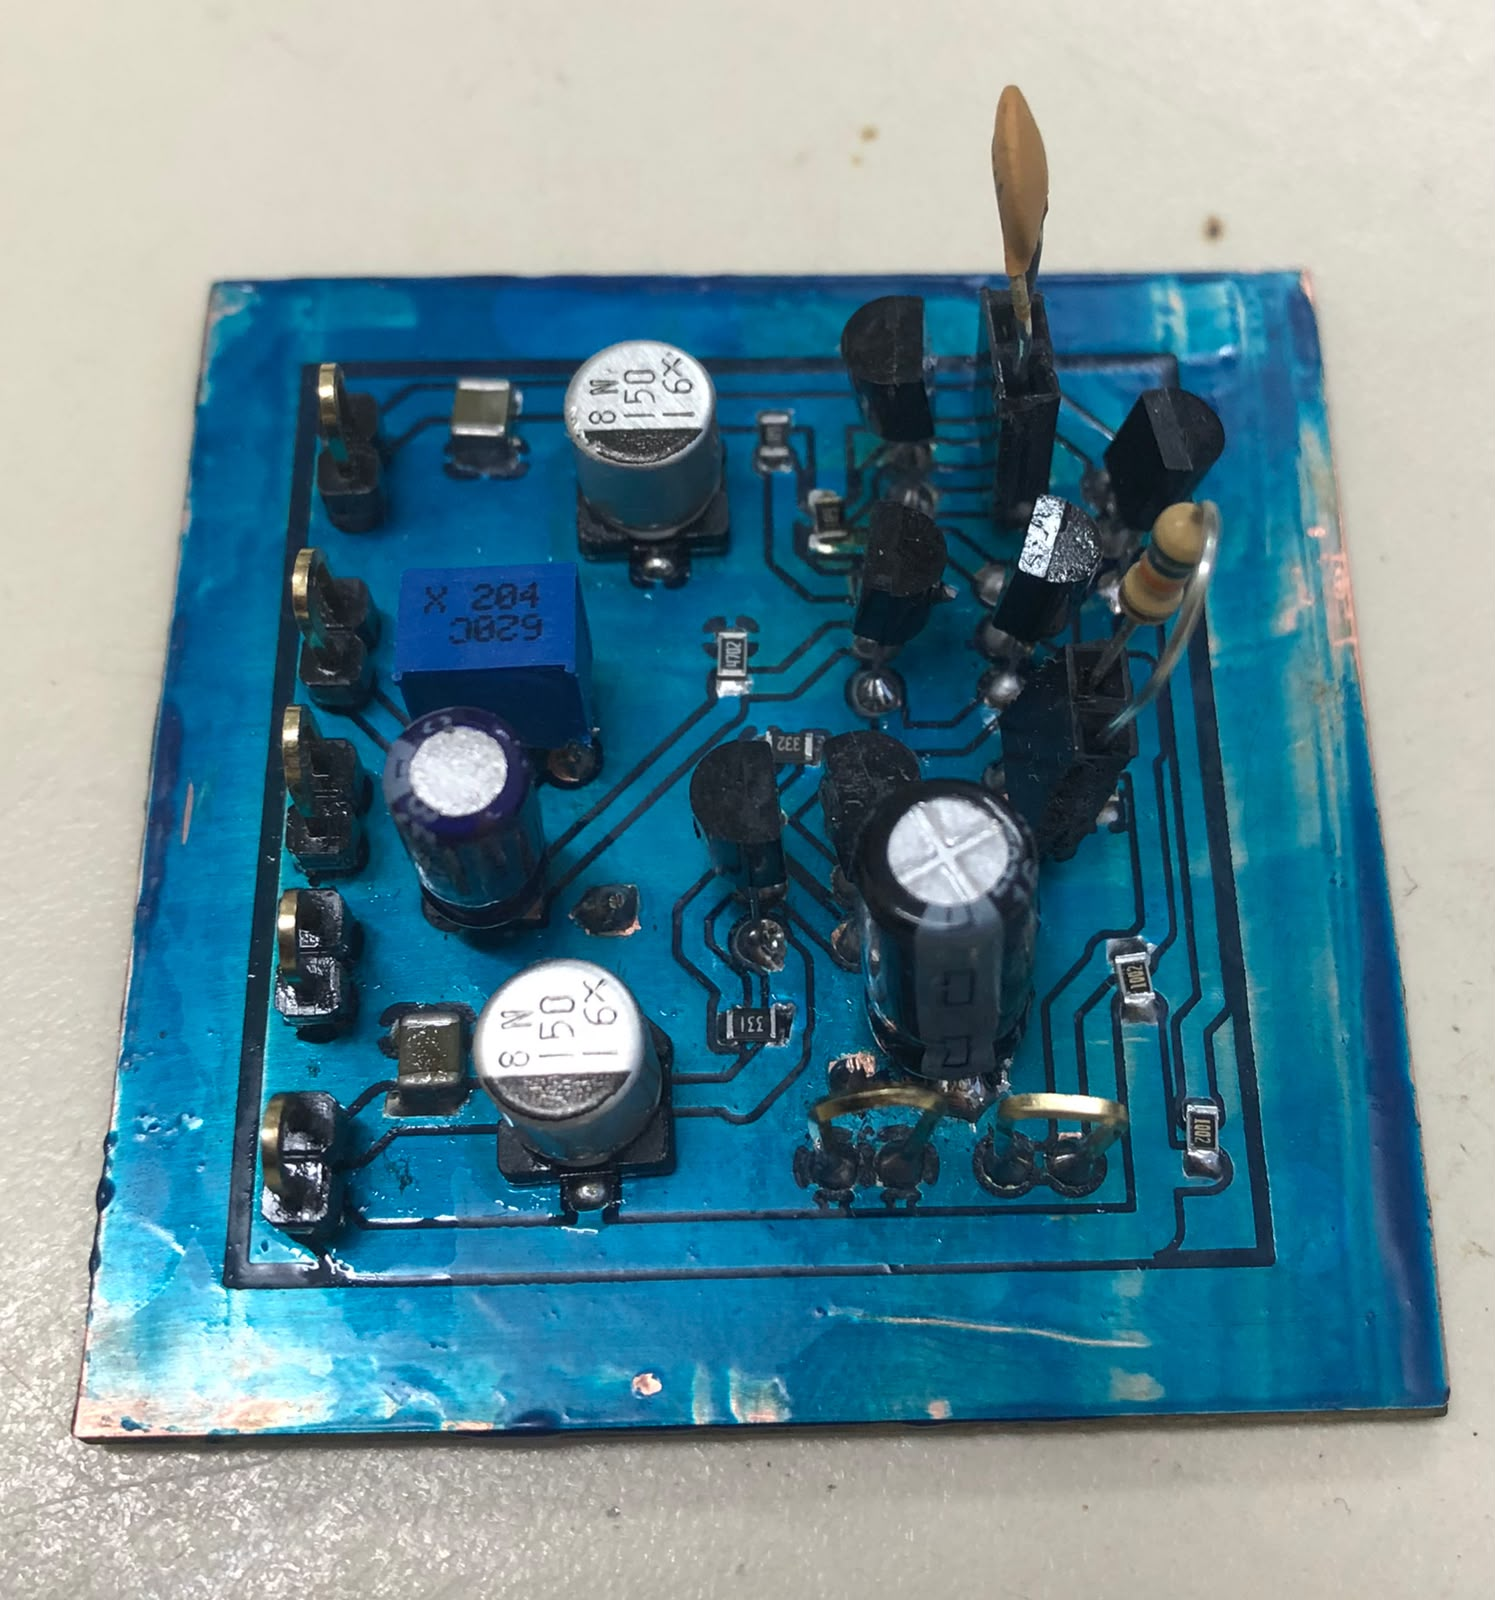
\includegraphics[width=7cm]{Fotos/Circuito1}
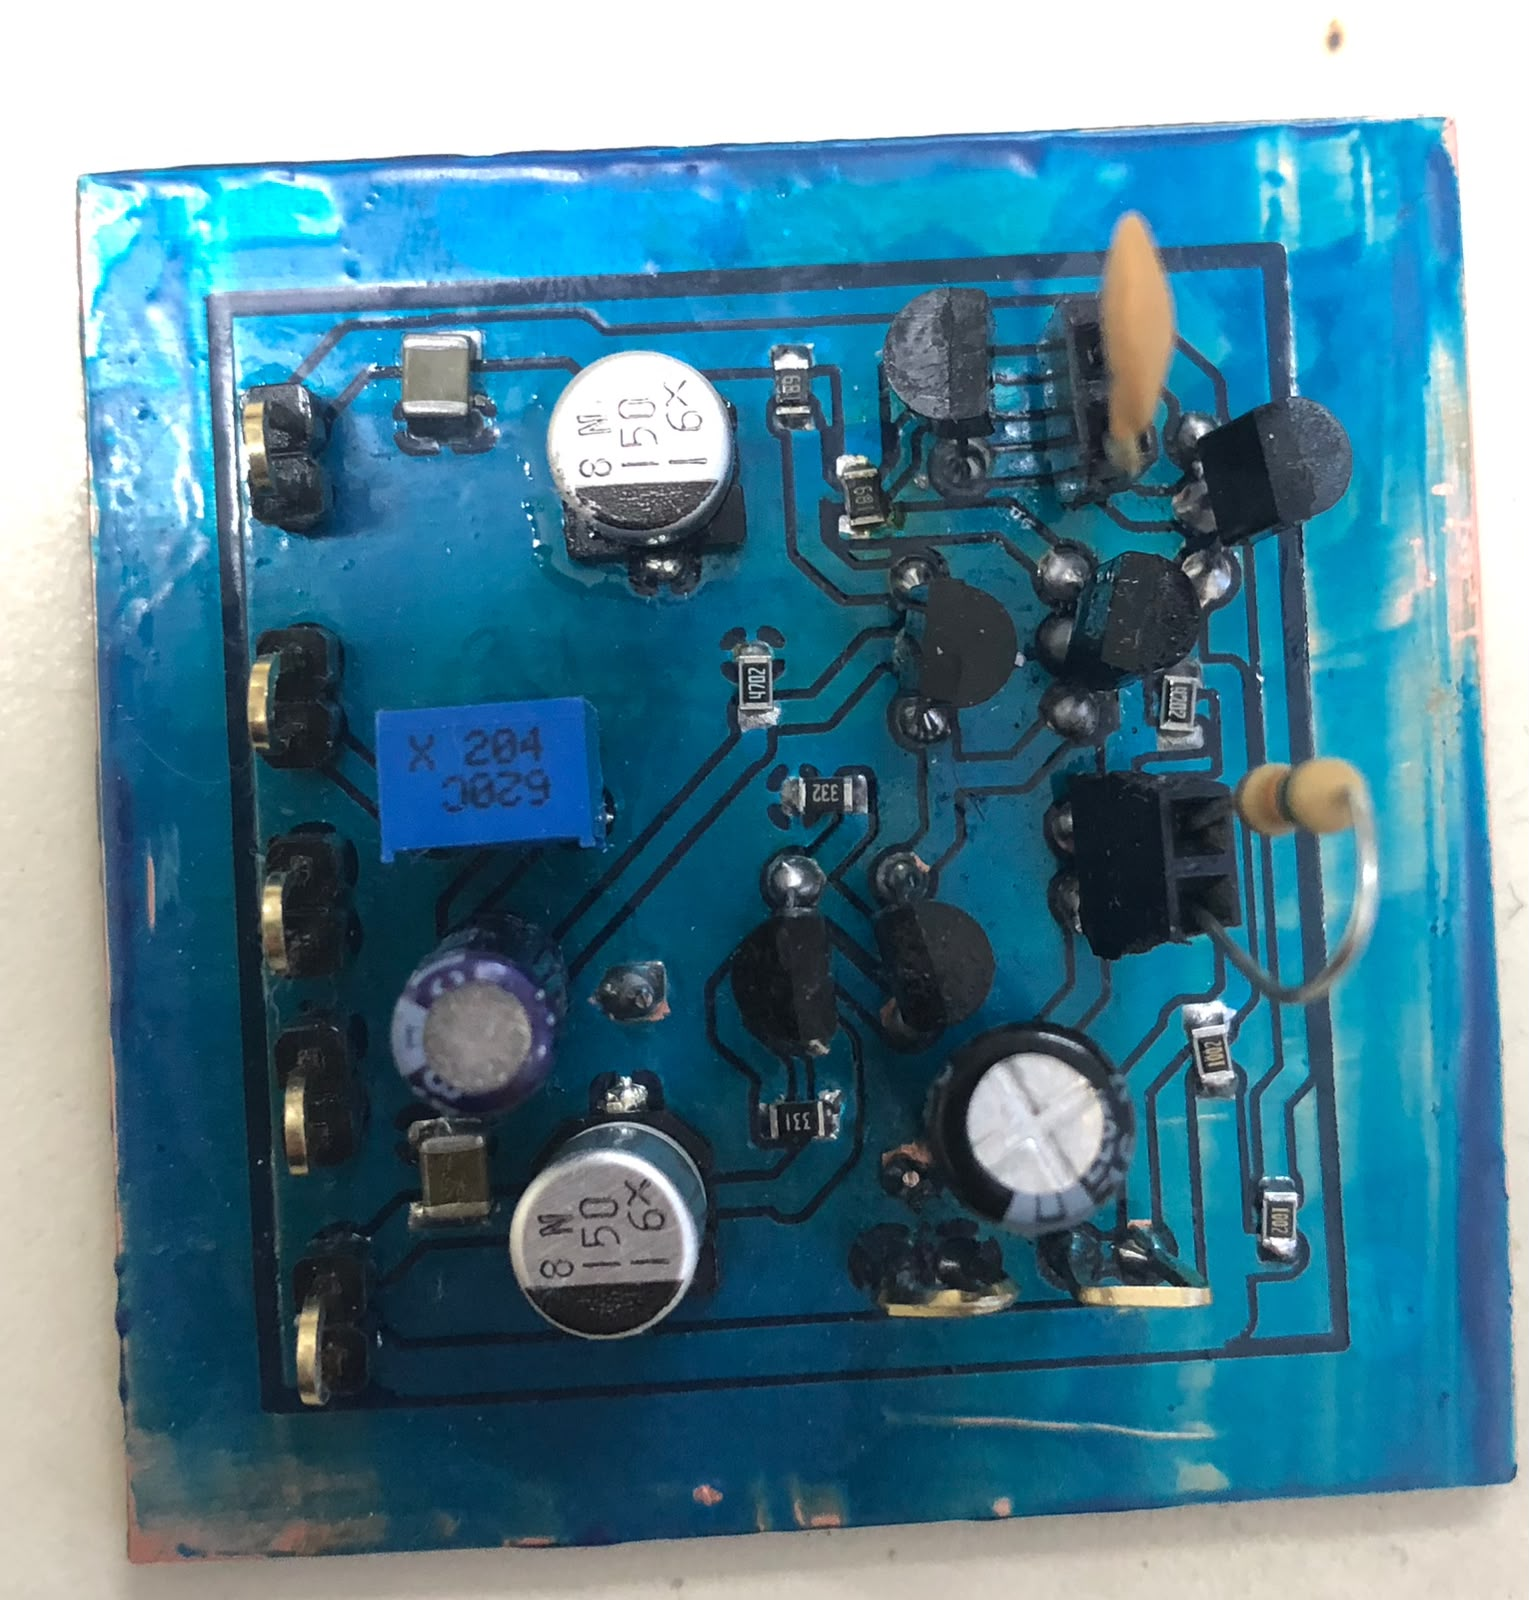
\includegraphics[width=7cm]{Fotos/Circuito2}
\caption{Circuito armado}
\end{figure}

\section{Calculos Teoricos (2)}
\subsection{Calculos Continua} \label{sec:calccc}

Se calcula el punto de trabajo del circuito de continua (fig \ref{fig:scheCont}), cuyos valores se vuelcan en la tabla comparativa (tab \ref{tab:cc}). Para este analisis se anulan las fuentes de señal y los capacitores se reemplazan por circuitos abiertos, de modo que solo permanecen las fuentes de alimentacion \(V_{cc}\) y \(V_{ee}\) y la red resistiva de polarizacion. Se adopta para las junturas base-emisor una tension \(V_{BE}\) de entre 0.65V y 0.75V, y se desprecian las corrientes de base frente a las de colector, lo cual es razonable dados los valores de \(h_{fe}\) del orden de 300.

\begin{figure}[h!]
    \centering
    \includestandalone[width=11cm]{CircCont}
    \caption{Circuito de Continua}
    \label{fig:scheCont}
\end{figure}

Se comienza por la fuente de corriente que polariza el par diferencial, formada por \(Q_3\) y \(Q_4\). La tension sobre \(R_{E3}\) queda fijada por la juntura base-emisor de \(Q_4\), y a partir de ella se obtiene la corriente de colector de \(Q_3\).

\begin{equation}
V_{R_{E3}} = V_{e_3} - V_{ee} = V_{BE_4} = 0.65V
\end{equation}
\begin{equation}
V_{e_3} = V_{ee} + V_{BE_4} = -8.35
\end{equation}
\begin{equation}
I_{CQ_3} = I_{R_{E3}} = \frac{V_{R_{E3}}}{R_{E3}} = 1.97mA
\end{equation}
Dado que el par diferencial es simetrico, la corriente que entrega la fuente se reparte en partes iguales entre \(Q_1\) y \(Q_2\).

\begin{equation}
I_{CQ_1} = I_{CQ_2} = \frac{I_{CQ_3}}{2} = 0.98 mA
\end{equation}
A continuacion se determina el punto de operacion de \(Q_4\). Su tension colector-emisor es la suma de las tensiones base-emisor de \(Q_3\) y \(Q_4\), y su corriente de colector se obtiene de la caida sobre \(R_{B3}\), ya que la corriente de base de \(Q_3\) es despreciable frente a la que circula por dicha resistencia.

\begin{equation}
V_{CEQ_4} = V_{BE_3} + V_{BE_4}  = 1.35V
\end{equation}
\begin{equation}
-V_{c4} = V_{ee} + V_{CEQ_4} = -7.64
\end{equation}
\begin{equation}
I_{CQ_4} \approx I_{R_{B3}} = \frac{-V_{c4}}{R_{B3}} = -\frac{V_{ee} + V_{CEQ_4}}{R_{B3}} = 2.31mA
\end{equation} 
Se analizan ahora las tensiones del par diferencial. Las bases de \(Q_1\) y \(Q_2\) se encuentran practicamente a 0V, ya que las corrientes de base son del orden de los microamperes y las caidas que producen en las resistencias conectadas a ellas son despreciables. En consecuencia, el emisor comun queda una tension \(V_{BE}\) por debajo de masa.

\begin{equation}
V_{b1} = I_{B_1} R_in \approx 0V
\end{equation}
\begin{equation}
V_{BE_1} = V_{BE_2} = 0.75V
\end{equation}
\begin{equation}
V_e = -V_{b1} - V_{BE_1} = -0.75
\end{equation}
\begin{equation}
V_{b2} = V_e + V_{BE_1} \approx 0V
\end{equation}
Conocidas las corrientes de colector, se calculan las tensiones de colector a partir de la caida sobre las resistencias de colector, y con ellas las tensiones colector-emisor de los transistores \(Q_1\), \(Q_2\) y \(Q_3\).

\begin{equation}
V_{c1} = V_{cc} - V_{R_C1} = V_{cc} - R_{C_1} I_{CQ_1} = 8.333V
\end{equation}
\begin{equation}
V_{c2} = V_{cc} - V_{R_C2} = V_{cc} - R_{C_2} I_{CQ_2} = 8.333V
\end{equation}
\begin{equation}
V_{CEQ_1} = V_{c1} - V_{e} = 9.08V
\end{equation}
\begin{equation}
V_{CEQ_2} = V_{c2} - V_{e} = 9.08V
\end{equation}
\begin{equation}
V_{CEQ_3} = V_{e} - V_{e3} = 7.6V
\end{equation}
Por ultimo se analiza la etapa de salida. La tension de continua en la salida \(V_o\) queda fijada practicamente en 0V, dado que la corriente de base de \(Q_2\) produce una caida despreciable sobre \(R_2\) (este punto se retoma en las consideraciones teoricas). Como el colector de \(Q_5\) esta conectado directamente a la base de \(Q_6\), su tension es la de salida mas una \(V_{BE}\), a partir de lo cual se obtienen las corrientes y tensiones de ambos transistores.

\begin{equation}
V_o = V_{b2} + V_{R_2} = V_{b2} + I_{B2} R_2 \approx 0V
\end{equation}
\begin{equation}
V_{c5} = V_o + V_{BE_6} = 0.(65V)
\end{equation}
\begin{equation}
I_{CQ_5} \approx -I_{R_{C_5}} = -\frac{V_{c5} - V_{ee}}{R_{C_5}} = -0.97mA
\end{equation}  
\begin{equation}
V_{CEQ_5} = V_{c5} - V_{cc} = -8.35V
\end{equation}
\begin{equation}
I_{CQ_6} = I_{R_{E_6}} = \frac{V_o - V_{ee}}{R_{E_6}} = 0.9mA
\end{equation} 
\begin{equation}
V_{CEQ_6} = V_{cc} - V_{o} = 9V
\end{equation}

\subsection{Circuito de Señal y Metodo Receta}

Para el analisis de pequeña señal se utiliza el modelo de parametros hibridos \(h_e\) de los transistores. A partir de las hojas de datos, a una corriente de colector de 2mA se obtienen, para ambos tipos de transistores utilizados, los siguientes valores:
\begin{equation}
hie = 4.5K; hfe=330; hoe=30\mu
\end{equation}

Como los transistores no operan a 2mA, estos parametros deben corregirse segun su corriente de colector real. Para ello se utilizan los graficos de la hoja de datos que muestran la variacion de cada parametro con la corriente de colector, normalizada respecto de su valor a 2mA, de los cuales se obtienen los factores de correccion \(f_c\) de la tabla (tab \ref{tab:fc}). Los transistores \(Q_3\) y \(Q_4\) operan a aproximadamente 2mA, por lo que sus factores son unitarios.

\begin{table}
\centering
\begin{tabular}{ |c|c|c|c|c| }\hline
Transistor         & \(\approx I_{CQ}\)[mA] & \(fc_{h_{ie}}\) & \(fc_{h_{ie}}\) & \(fc_{h_{ie}}\) \\\hline
\(Q_5           \) & -1                     & 1.8             & 0.97            & 0.5             \\\hline
\(Q_1, Q_2, Q_4 \) &  1                     & 2               & 0.95            & 0.6             \\\hline
\(Q_3, Q_4      \) &  2                     & 1               & 1               & 1               \\\hline
\end{tabular}
\caption{Factores de correccion \(\frac{h_e(I_c)}{h_e(2mA)}\)}
\label{tab:fc} 
\end{table}

Multiplicando los valores a 2mA por los factores de correccion se obtienen los parametros \(h_e\) de cada transistor en su punto de operacion, los cuales se resumen en la tabla (tab \ref{tab:he}) y se utilizan en el resto del analisis de señal.

\begin{table}
\centering
\begin{tabular}{ |c|c|c|c| }\hline
Transistor         & \(h_{ie}\) [\(K\Omega\)] & \(h_{fe}\) & \(h_{oe}\) [\(\mu S\)] \\\hline
\(Q_5           \) & 8.17                     & 320        & 15                     \\\hline
\(Q_1, Q_2, Q_4 \) & 9                        & 313        & 18                     \\\hline
\(Q_3, Q_4      \) & 4.5                      & 330        & 30                     \\\hline
\end{tabular}
\caption{Parametros \(h_e\)}
\label{tab:he} 
\end{table}

\subsubsection{Planteo Thevenin e Identifico Topologia de Red}

\begin{figure}[!h]
    \centering
    \includestandalone[width=11cm]{CircBasico}
    \caption{Circuito Original}
\end{figure}

Se identifica la topologia de la red de realimentacion. La red \(\beta\) toma muestra de la tension de salida \(V_o\) (se conecta en paralelo con la salida) y reinyecta en el lazo de entrada una tension \(V_f\) en serie con la fuente de señal, por lo que la topologia es Tension-Serie. Para esta topologia el cuadripolo de realimentacion se representa mediante parametros hibridos \(h\), y el amplificador basico se caracteriza por su ganancia de tension y sus resistencias de entrada y salida.

Podemos verificar que la realimentacion es negativa dado que la tension que llega a la entrada del amplificador basico es \( V_i = V_s - V_f \), es decir que la tension realimentada se resta a la tension de señal.

Del lado de la fuente, el equivalente de Thevenin se obtiene considerando la resistencia interna de la fuente de señal en paralelo con la resistencia de polarizacion de entrada \(R_{in}\), lo cual resulta aproximadamente igual a la resistencia de la fuente por ser \(R_{in}\) mucho mayor.

\begin{equation}
{R_{th}} = 50 \Omega \parallelsum 47K\Omega \approx 50 \Omega
\end{equation}

\subsubsection{\texorpdfstring{Parametros de  Red \(\beta\)}{Parametros de Red }}

La red de realimentacion, formada por \(R_1\) y \(R_2\), se modela como un cuadripolo mediante sus parametros hibridos \(h\), como se muestra en la siguiente figura.

\begin{figure}[h!]
    \centering
    \includestandalone[width=5cm]{Beta}
    \caption{Cuadripolo de la Malla \(\beta\)}
\end{figure}

Los parametros del cuadripolo se calculan con \(R_1 = 4.7K\Omega\) y \(R_2 = 47K\Omega\). El parametro \(h_{11}\) es la resistencia que la red presenta a la entrada con la salida en cortocircuito, y representa el efecto de carga de la red sobre la entrada del amplificador. El parametro \(h_{12}\) es la transferencia inversa de tension, que corresponde al factor de realimentacion \(\beta\). Por ultimo, \(h_{22}\) es la admitancia de salida de la red, que representa su efecto de carga sobre la salida del amplificador. Se desprecia la transmision directa \(h_{21}\) de la red, por ser esta pasiva y mucho menor que la ganancia del amplificador.

\begin{equation}
h_{11} = \left. \frac{V_1}{I_1} \right\vert_{V_2 = 0} = R_2 \parallelsum R_1 = 4.27 K\Omega 
\end{equation}
\begin{equation}
h_{12} = \left. \frac{V_1}{V_2} \right\vert_{I_1 = 0} = \frac{R_1}{R_1 + R_2} = 90.91 \cdot 10^{-3} 
\end{equation}
\begin{equation}
h_{22} = \left. \frac{I_2}{V_2} \right\vert_{I_1 = 0} = \frac{1}{R_1 + R_2} = (51.7 K\Omega)^{-1} 
\end{equation}

\subsubsection{Armado del NAB}

Se arma el Nuevo Amplificador Basico (NAB), que incorpora al amplificador a lazo abierto los efectos de carga de la red \(\beta\): \(h_{11}\) se agrega en serie a la entrada y \(\frac{1}{h_{22}}\) se coloca en paralelo con la salida. Sobre este circuito se calculan la resistencia de entrada \(R_{is}\), la resistencia de salida \(R_{os}\) y la ganancia de tension sin realimentar \(A_{vs}\).

\begin{figure}[h!]
    \centering
    \includestandalone[width=11cm]{NAB}
    \caption{Nuevo Amplificador Basico}
\end{figure}

La resistencia de entrada sin realimentar incluye la resistencia de la fuente, \(h_{11}\) y las resistencias \(h_{ie}\) de \(Q_1\) y \(Q_2\), ya que en el par diferencial la señal atraviesa las dos junturas base-emisor en serie.

\begin{equation}
R_{is} = R_s + 2 h_{ie_{12}} + h_{11} 
\end{equation}
\begin{equation}
h_{ie_{12}} = 9K\Omega
\end{equation}
\begin{equation}
h_{fe_{12}} = 313
\end{equation}
\begin{equation}
R_{is} = R_s + 2 h_{ie} + h_11 = 50\Omega + 2 \cdot 9K\Omega + 4.27 K\Omega  = 22.27K\Omega 
\end{equation}
Para la resistencia de salida se consideran en paralelo la carga \(R_L\), la resistencia \(R_{E6}\), la admitancia \(h_{22}\) de la red de realimentacion y la resistencia de salida del seguidor de emisor \(Q_6\). Esta ultima es mucho menor que el resto, por lo que domina el resultado.

\begin{equation}
R_{os} = R_L \parallelsum R_{E6} \parallelsum \frac{1}{h_{22}} \parallelsum R_{O_{Q6}}
\end{equation}
\begin{equation}
h_{oe_{5}} 15 \mu S
\end{equation}
\begin{equation}
R_{O_{Q5}} = \frac{1}{15 \mu S} = 66.66K\Omega
\end{equation}
\begin{equation}
R_{O_{Q6}} = \frac{h_{ie_{6}}}{h_{fe_{6}}} + \frac{R_{C5} \parallelsum R_{O_{Q6}}}{1 + h_{fe_{6}}} = \frac{9K\Omega}{314} + \frac{10K\Omega \parallelsum 66.6K\Omega}{314} = 56.35\Omega
\end{equation}
\begin{equation}
R_{os} = 47K\Omega \parallelsum 10K\Omega \parallelsum 51.7K\Omega \parallelsum 56.35\Omega \approx 56.35\Omega
\end{equation}
\par
La ganancia de tension sin realimentar se obtiene como el producto de las ganancias de las tres etapas: el seguidor de emisor de salida (\(Q_6\)), la etapa amplificadora con \(Q_5\) y la etapa diferencial de entrada. El seguidor presenta una ganancia aproximadamente unitaria, por lo que la mayor parte de la ganancia proviene de las otras dos etapas.

\begin{equation}
A_{vs} = \frac{V_O}{V_S} = \frac{V_O}{V_X} \cdot \frac{V_X}{V_Y} \cdot \frac{V_Y}{V_S} 
\end{equation}
\begin{equation}
\frac{V_O}{V_X} = \frac{ \left( 1 + h_{fe_{6}} \right) \left( R_{e6} \parallelsum R_L \parallelsum \frac{1}{h_{22}} \right)}{h_{ie_{6}} + \left( 1 + h_{fe_{6}} \right) \cdot \left( R_{e6} \parallelsum R{L} \parallelsum \frac{1}{h_{22}} \right)} = \frac{ 314 \cdot 7.111K\Omega}{9K\Omega + 314 \cdot 7.111K\Omega} \approx 1 
\end{equation}
\begin{equation}
\frac{V_X}{V_Y} = -gm_5 \left( R_{c5} \parallelsum R_{iQ6} \right) \approx -40V^{-1} \cdot 0.97mA \cdot 10K\Omega = -388
\end{equation}
\begin{equation}
\frac{V_Y}{V_S} = 
\frac{-h_{fe_{1}} \left( R_{C1} \parallelsum R_{is} \parallelsum R_{O_{Q1}} \right) }{R_s + 2 h_{ie_{1}} + h_{11}} = 
\frac{-313 \left( 680\Omega \parallelsum 9K\Omega \Omega \right)}{50\Omega + 2 \cdot 9K\Omega + 4.27K\Omega} = -8.86 
\end{equation}
\begin{equation}
A_{vs} = 0.65 \cdot (-388) \cdot (-9.45) = 3440
\end{equation}

\subsubsection{Calculo de los Parametros Realimentados y Fin del Metodo Receta}\label{sec:CalcXvsf}

Se calculan a continuacion los parametros \(A_{vsf}\), \(R_{isf}\) y \(R_{osf}\), los mismos se vuelcan en la tabla comparativa (tab \ref{tab:xsf}). Para ello se calcula primero el factor de realimentacion \(D = 1 + A_{vs} \beta\), que indica cuanto se modifican las caracteristicas del amplificador al realimentarlo. La ganancia realimentada resulta aproximadamente \(\frac{1}{\beta}\), la resistencia de entrada se multiplica por \(D\) y la de salida se divide por \(D\), tal como corresponde a la topologia Tension-Serie.

\begin{equation}
D = 1 + (A_{vs} \cdot \beta) = 313.7
\end{equation}
\begin{equation}
A_{vsf} = \frac{A_{vs}}{D} = 10.96
\end{equation}
\begin{equation}
R_{isf} = R_{is} \cdot D = 6.98M\Omega; R_{in} \parallelsum R_{isf} \approx R_{in} 
\end{equation}
\begin{equation}
R_{osf} = \frac{R_{os}}{D} = 0.17\Omega
\end{equation}

Se observa que \(R_{isf}\) resulta muy elevada, por lo que la resistencia de entrada del circuito completo queda determinada practicamente por \(R_{in}\). Por su parte, \(R_{osf}\) es del orden de las decimas de ohm, con lo cual la salida se comporta de forma muy cercana a una fuente de tension ideal.

\newpage

\newpage
\section{Simulaciones}

En esta seccion se presentan las simulaciones realizadas en LTspice, utilizando los esquematicos de las figuras (fig \ref{fig:scheGen}) y (fig \ref{fig:scheRo}). El primero se emplea para obtener el punto de operacion de continua, la respuesta en frecuencia, \(A_{vsf}\) y \(R_{isf}\), y para las variaciones del capacitor de compensacion y de \(R_1\). El segundo es una version modificada del circuito que se utiliza para obtener \(R_{osf}\). Los resultados se contrastan con los valores calculados y medidos en la seccion de tablas comparativas.

\begin{figure}[h!]
\centering
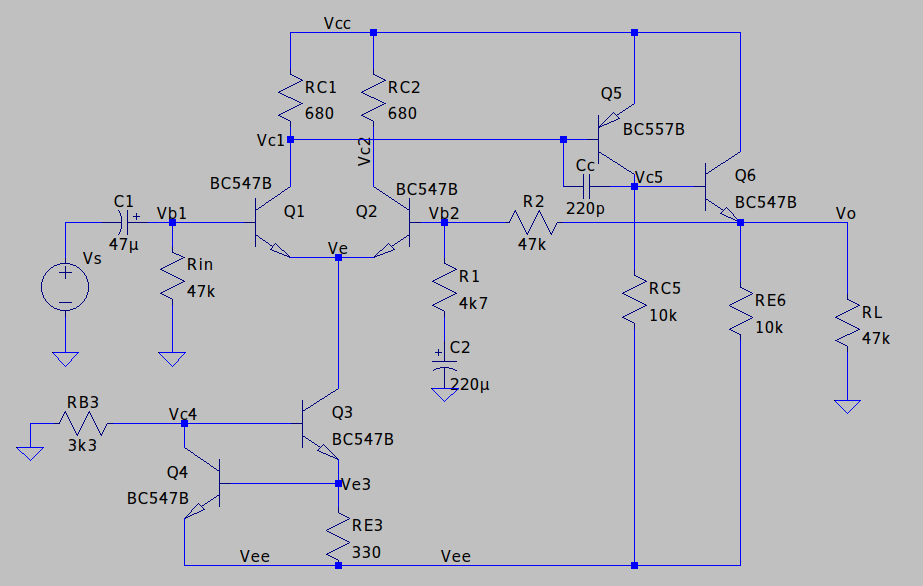
\includegraphics[width=11cm]{Sche/Gen.png}
\caption{Esquematico Utilizado para la simulacaion de continua, \(A_{vsf}\) y \(R_{isf}\), variaciones de \(C_c\)}
\label{fig:scheGen}
\end{figure}

\begin{figure}[h!] 
\centering
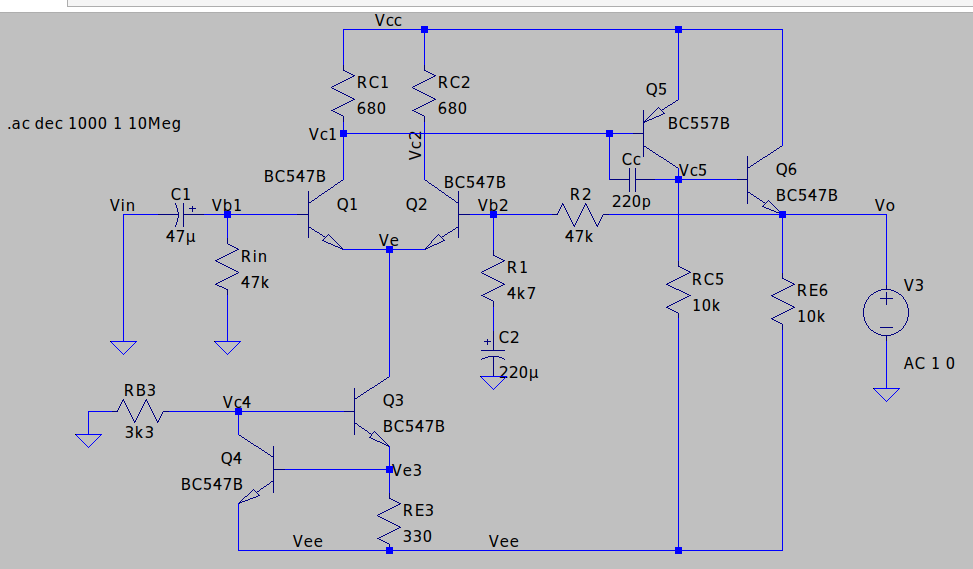
\includegraphics[width=11cm]{Sche/Ros.png}
\caption{Esquematico Utilizado para la simulacaion de \(R_{osf}\)}
\label{fig:scheRo}
\end{figure}

\subsection{Punto de operacion en continua (3)} \label{sec:simcc}
Se tomaron las medidas del punto de operacion utilizando la instruccion .op, que resuelve el circuito en continua con las fuentes de señal anuladas. Las mismas se encuentran en la tabla comparativa de valores (tab \ref{tab:cc}). Se observa una muy buena concordancia con los valores calculados: las tensiones colector-emisor difieren en menos de 0.1V y las corrientes de colector coinciden, salvo por la asimetria entre \(Q_1\) y \(Q_2\) (0.91mA y 1.09mA). Esta asimetria no aparece en el calculo, que supone un par diferencial perfectamente simetrico y desprecia las caidas por corrientes de base, y se debe en parte a que las resistencias conectadas a las bases (\(R_{in}\) en \(Q_1\) y \(R_1 \parallelsum R_2\) en \(Q_2\)) son distintas, por lo que dichas caidas no son iguales en ambos transistores. 

\subsection{\texorpdfstring{\(A_{vsf}\), \(R_{isf}\) y \(R_{osf}\) (4)}{, y (4)}} \label{sec:SimXvsf}

\begin{figure}[ht] 
\centering
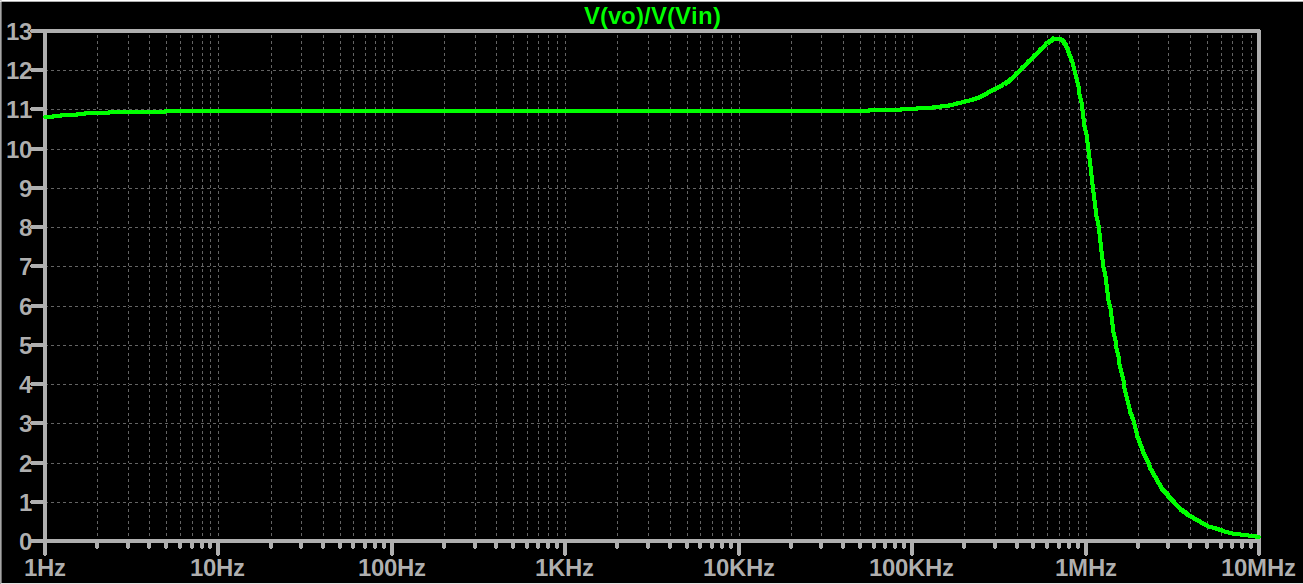
\includegraphics[width=9cm]{Plot/Avsf.png} \\
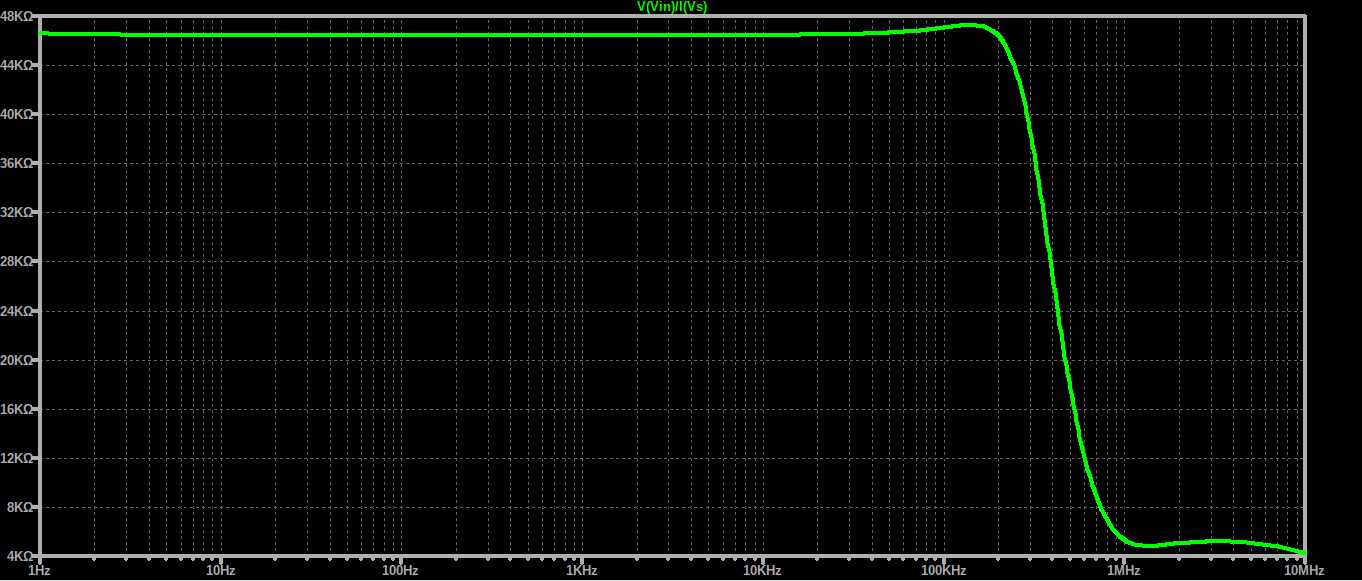
\includegraphics[width=9cm]{Plot/RisfPlot.png} \\
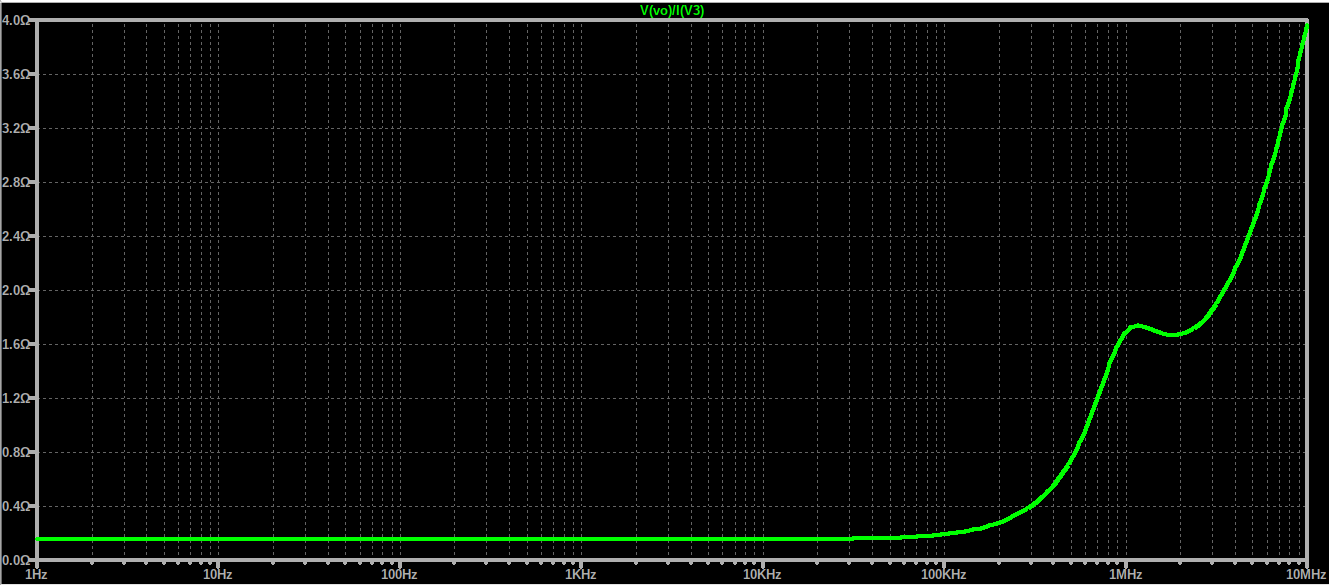
\includegraphics[width=9cm]{Plot/RosfPlot.png}
\caption{(de arriba hacia abajo) Plots de \(A_{vsf}\), \(R_{isf}\) y \(R_{osf}\)}
\label{fig:.ac}
\end{figure}

Con la instruccion .ac se toman los plots de \(A_{vsf} (V(Vo)/V(Vin))\) y \(R_{isf} (V(Vin)/I(Vin))\) del esquematico original (fig \ref{fig:scheGen}), asi como el valor de \(R_{osf} (V(Vin)/I(V3))\) del esquematico modificado (fig \ref{fig:scheRo}), obteniendo los plots de estos parametros (fig \ref{fig:.ac}). Los valores se encuentran en la tabla comparativa (tab \ref{tab:xsf}). La ganancia simulada (10.96) coincide con la calculada (10.95), lo que valida el calculo realizado con el metodo de la receta. La \(R_{isf}\) simulada (46.47K\(\Omega\)) es muy cercana a \(R_{in}\) = 47K\(\Omega\), debido a que la resistencia de entrada realimentada del amplificador es de varios megaohms y por lo tanto la resistencia vista por la fuente queda dominada por \(R_{in}\). Finalmente, la \(R_{osf}\) simulada (155m\(\Omega\)) es del mismo orden que la calculada (170m\(\Omega\)), confirmando que la realimentacion reduce la resistencia de salida a valores muy bajos.

\subsection{Variaciones en el Capacitor de compensacion (10)} \label{sec:cc}

\begin{figure}[ht] 
\centering
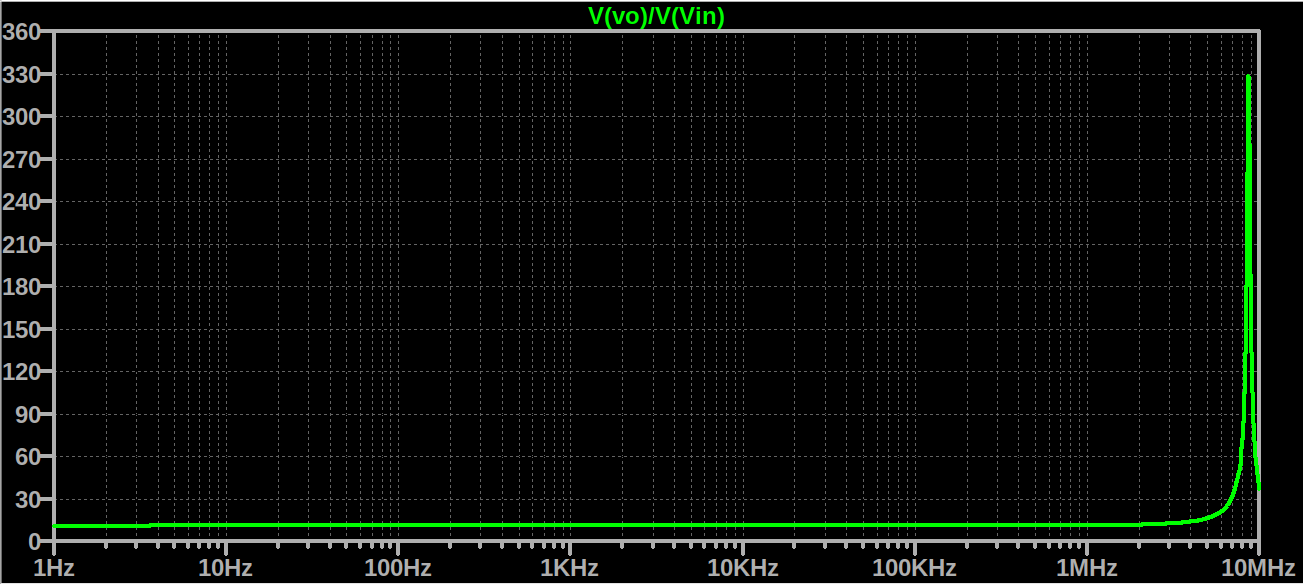
\includegraphics[width=9cm]{Plot/AvsfSinCC.png} \\
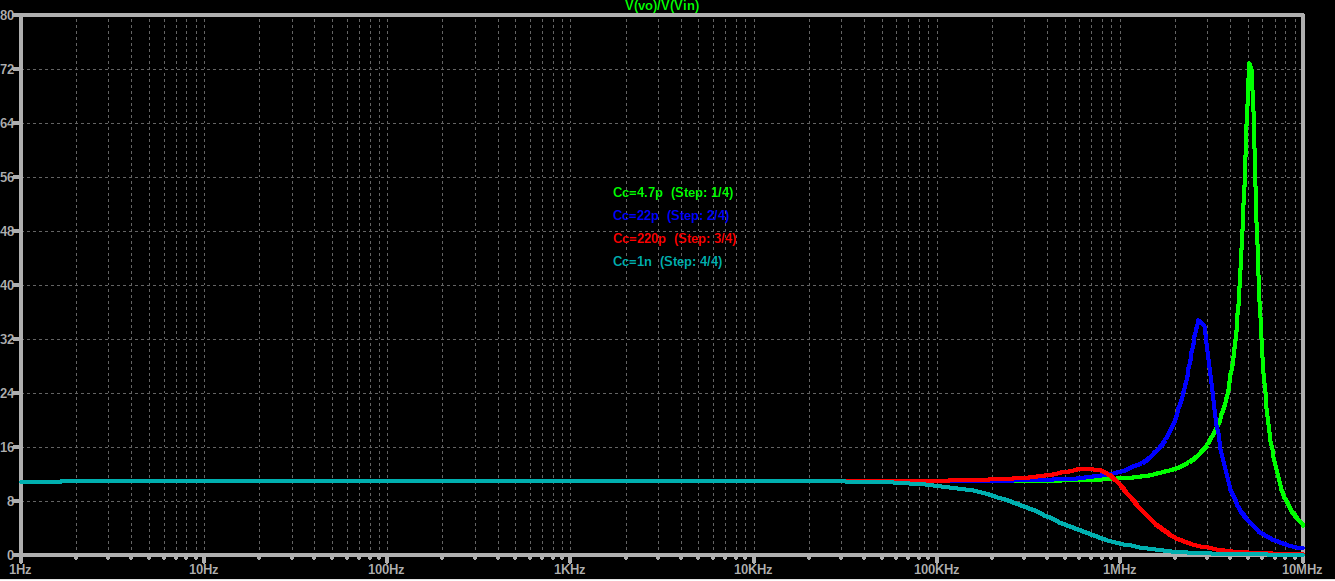
\includegraphics[width=9cm]{Plot/AvsfCCParam.png} 
\caption{(de arriba hacia abajo) Plot con el capacitor de compensacion removido, plot con el capacitor de compensacion parametrizado en 4.7pF, 22pF, 220pf y 1nf.}
\label{fig:capsweep}
\end{figure}

Al remover el capacitor de compensacion puede observarse en los plots resultantes (fig \ref{fig:capsweep}) que aparece un gran sobrepico a altas frecuencias. Este se debe a un componente de realimentacion positiva que surje a estas frecuencias: cada etapa del amplificador introduce polos que agregan desfasaje a medida que aumenta la frecuencia, y cuando el desfasaje acumulado en el lazo se acerca a 180° la realimentacion, que a frecuencias medias es negativa, se vuelve positiva. Si en ese rango la ganancia de lazo sigue siendo cercana o mayor a la unidad, se produce un sobrepico en la respuesta, que en el caso extremo se traduce en oscilacion. El capacitor de compensacion introduce un polo dominante a baja frecuencia que reduce la ganancia de lazo antes de que el desfasaje llegue a 180°, mejorando el margen de fase. Al agregar el capacitor se puede observar que el pico de sobreamplificacion se reduce y se mueve hacia las bajas frecuencias. Este efecto es mayor cuanto mayor es el valor del capacitor. Si el valor es demasiado elevado, empieza a recortarse el ancho de banda del amplificador. Los valores se vuelcan en la tabla (tab \ref{tab:cap}), donde se indica para cada valor de \(C_c\) la frecuencia a la que se produce el pico de ganancia y su amplitud. Al aumentar la capacidad el pico se desplaza hacia frecuencias menores y su amplitud disminuye. Con 1nF el sobrepico desaparece (la ganancia de 10.31 es inferior a la de banda media), pero a costa de un ancho de banda considerablemente recortado. De esta forma, el valor de 220pF resulta un compromiso adecuado entre la reduccion del sobrepico y el mantenimiento del ancho de banda.


\begin{table}
\centering
\begin{tabular}{ |c|c|c| } \hline
Valor de \(C_c\) [pF] & \(\omega\) [KHz] & \(A(\omega)\) \\ \hline         
0                     & 8689             & 332.25        \\ \hline 
4.7                   & 5152             & 73.85         \\ \hline 
22                    & 2739             & 35.30         \\ \hline 
220                   & 674.5            & 12.83         \\ \hline 
1000                  & 101.6            & 10.31         \\ \hline 
\end{tabular}
\caption {Parametros de operacion de Señal}
\label{tab:cap} 
\end{table}

\subsection{\texorpdfstring{Variaciones en la Resistencia \(R_1\) (11)}{Variaciones en la Resistencia (11)}} \label{sec:simR1}

\begin{figure}[ht] 
\centering
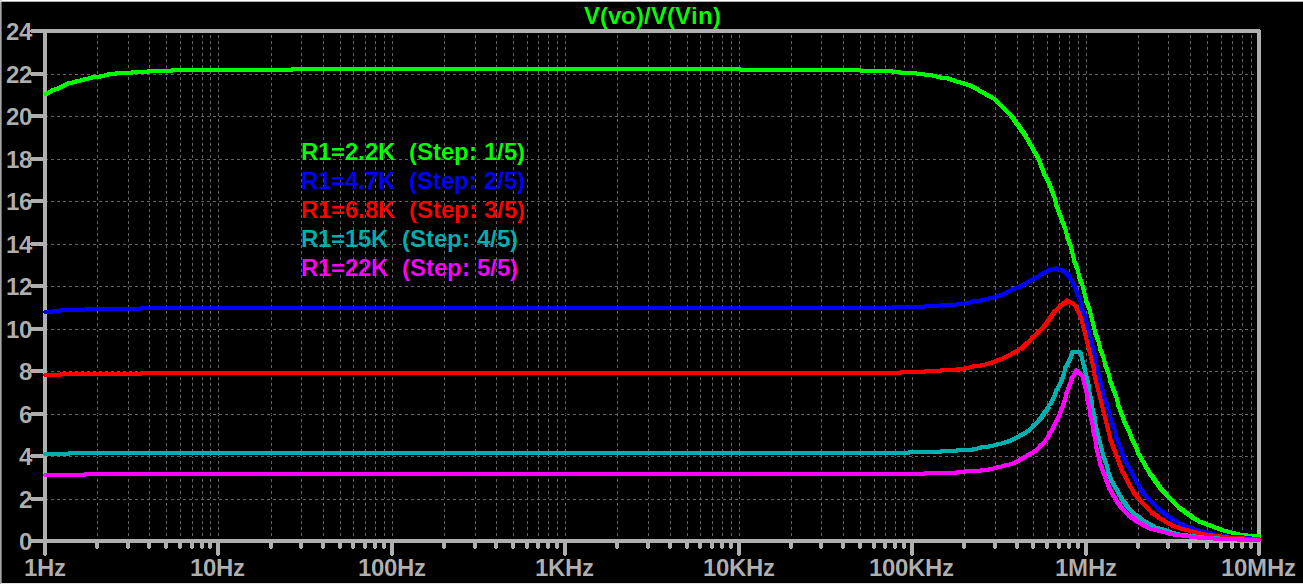
\includegraphics[width=11cm]{Plot/AvsfR1param.png}
\caption{Plot con la resistencia \(R_1\) parametrizada en \(2.2K\Omega\), \(4.7K\Omega\), \(6.8K\Omega\), \(15K\Omega\) y \(22K\Omega\).}
\label{fig:R1}
\end{figure}

Podemos aproximar la ganancia de la siguiente manera.

\begin{equation}
A_{vsf} = \frac{A_vs}{1 + A_{vs} \cdot \beta} \approx \frac{1}{\beta} = 1 + \frac{R_2}{R_1}
\end{equation}

De esta forma, podemos esperar que al reducir \(R_1\) aumente \(A_{vsf}\). En el plot obtenido de realizar esta variacion (fig \ref{fig:R1}) se puede comprobar este fenomeno. Los valores obtenidos de la simulacion y los calculados de esta forma se vuelcan en la tabla (tab \ref{tab:R1}). Los valores simulados difieren en menos de 1\% de los calculados. Los valores calculados resultan levemente mayores, lo cual es esperable ya que \(\frac{1}{\beta}\) es el limite al que tiende la ganancia realimentada cuando la ganancia de lazo es infinita, pero en la realidad esta es finita.

\newpage
\section{Proceso de Medicion}
Para la realizacion de las mediciones utilizamos un osciloscopio Siglent SDS 2204X, un generador de señales Twintex TFG-3205E y una Red Pitaya 125-14. A continuacion se describe el procedimiento seguido en cada una de las mediciones y los resultados obtenidos, que luego se comparan con los valores calculados y simulados en la seccion de tablas comparativas.

\begin{figure}[ht] 
\centering
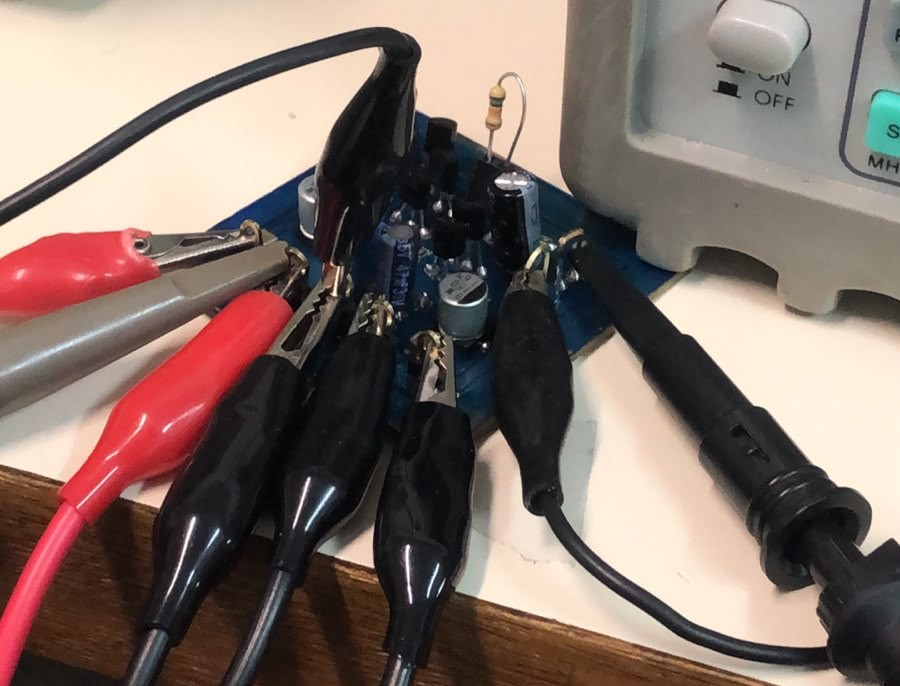
\includegraphics[width=11cm]{Fotos/Med}
\caption{Banco de Mediciones}
\end{figure}

\subsection{Medicion del punto de polarizacion de los transistores (5), (6)} \label{sec:medcc}

%\begin{figure}[ht] 
%\centering
%\includegraphics[width=11cm]{Fotos/CC}
%\caption{Medicion del punto de trabajo}
%\end{figure}

Se midio el punto de trabajo de los transistores con tension de \({V_{CC} = 8.984}\), \({V_{EE} = -9.129}\) y \({V_{O} = 0,0078V}\). Los mismos se encuentran volcados en la tabla comparativa (tab \ref{tab:cc}). Las tensiones de alimentacion reales difieren ligeramente de los \(\pm 9V\) nominales utilizados en el calculo, lo que explica parte de las pequeñas diferencias entre los valores medidos y calculados. Se destaca que la tension continua de salida resulto de apenas 7.8mV, es decir practicamente nula, tal como predice la teoria (ver consideraciones teoricas). Salvo por \(Q_2\), cuya corriente de colector (1.354mA) es considerablemente mayor a la calculada (0.98mA), las corrientes medidas difieren en menos de 8\% de las calculadas, y las tensiones colector-emisor lo hacen en menos de 0.25V. La asimetria entre las corrientes de \(Q_1\) y \(Q_2\) puede atribuirse a la dispersion de parametros entre los transistores y a la diferencia entre las resistencias conectadas a sus bases, como se analizo en las simulaciones. 


\subsection{\texorpdfstring{Medicion de \(A_{vsf}\) (7)}{Medicion de  (7)}} \label{sec:MedAvsf}

\begin{figure}[ht] 
\centering
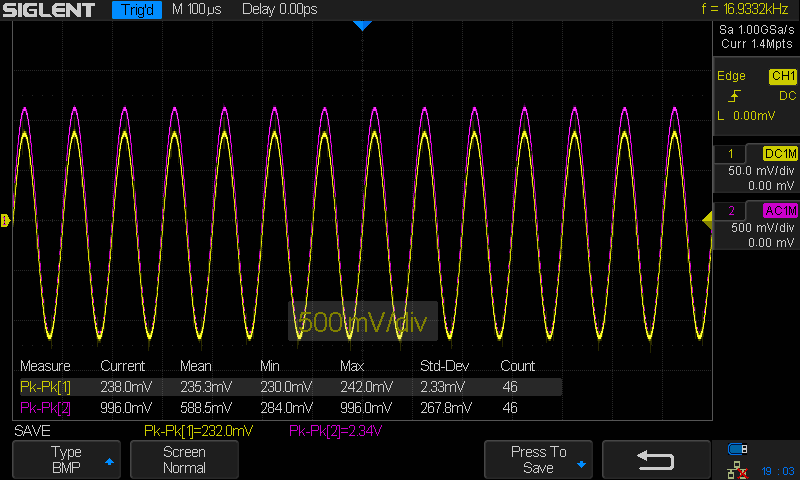
\includegraphics[width=11cm]{Osci/Avsf}
\caption{Oscilograma correspondiente a la medicion de \(A_{vsf}\)}
\end{figure}

Se aplico una \(V_s\) senoidal de 10KHz de frecuencia y 200mVpp, la ganancia obtenida es volcada en la tabla comparativa (tab \ref{tab:xsf}). Se eligio una frecuencia ubicada en la banda media del amplificador y una amplitud pequeña, de modo que la salida (de aproximadamente 2.2Vpp) se mantenga lejos de la saturacion y sin distorsion apreciable. La ganancia se obtiene como el cociente entre las amplitudes pico a pico de salida y entrada. El valor medido (10.849) difiere en aproximadamente 1\% del calculado y del simulado, lo cual confirma que la ganancia realimentada queda fijada por la red \(\beta\).

\subsection{\texorpdfstring{Barrido de frecuencia y obtension de \(A_{vsf}(\omega)\) (8) y (9)}{Barrido de frecuencia y obtension de }}

\begin{figure}[ht] 
\centering
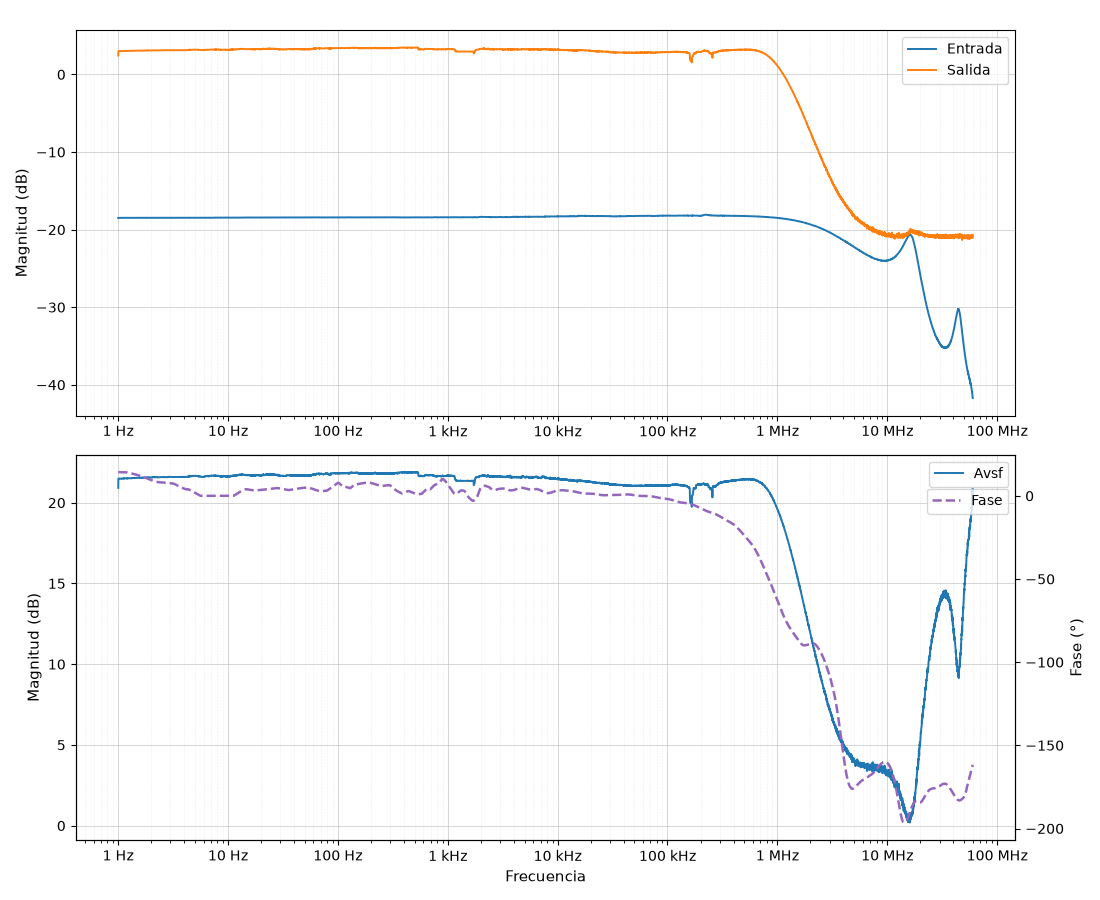
\includegraphics[width=16cm]{Plot/AvsfMed}
\caption{(arriba) \(A_{V_I}\) y \(A_{V_O}\) en barrido de frecuencia\\
(abajo)  \(A_{vsf}\) en barrido de frecuencia, modulo y fase}
\label{fig:barrido}
\end{figure}

Realizando un barrido de frecuencia desde 1Hz hasta 60MHz
se obtuvo \(A_{vsf}(\omega)\). A frecuencias superiores a 10MHz se empieza a reducir la amplitud en el generador de señales. Como a esas frecuencias la tension de salida ya se encuentra por debajo del piso de ruido (Y por ende la tension de salida medida no puede bajar mas), se aparenta un aumento ficticio de la ganancia del amplificador. Puede observarse el polo en 10MHz y una variacio de -180° alrededor de la frecuencia del polo (fig \ref{fig:barrido}). Dentro de la banda de paso se espera que la ganancia sea aproximadamente constante e igual a \(A_{vsf}\), y el polo determina el limite superior del ancho de banda del amplificador. El aumento ficticio de la ganancia por encima de los 10MHz se explica porque la ganancia se calcula como el cociente entre la tension de salida y la de entrada: al reducirse la amplitud de entrada mientras la salida permanece en el piso de ruido, el cociente crece aunque el amplificador no este amplificando realmente.

\subsection{Variacion de CC (10)}

\begin{figure}[ht] 
\centering
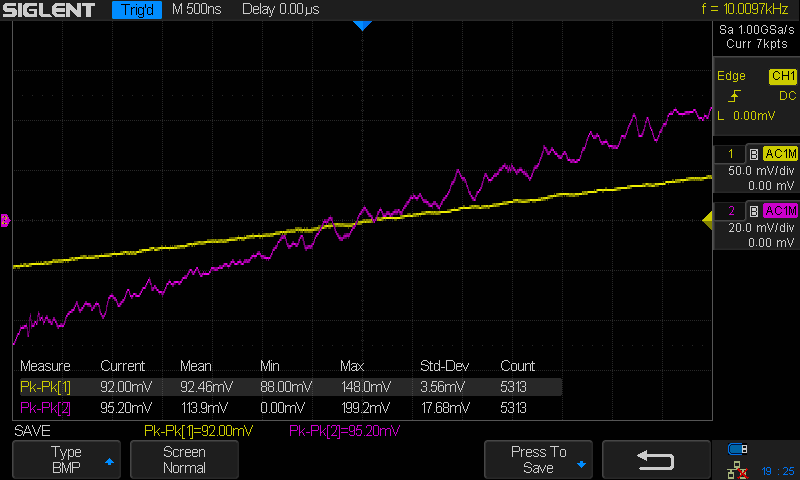
\includegraphics[width=7cm]{Osci/AvsfCC4p7}
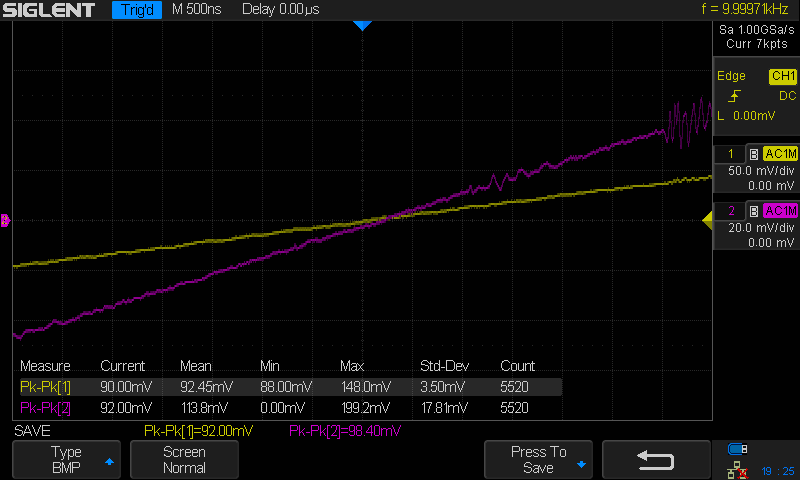
\includegraphics[width=7cm]{Osci/AvsfCC22p} \\
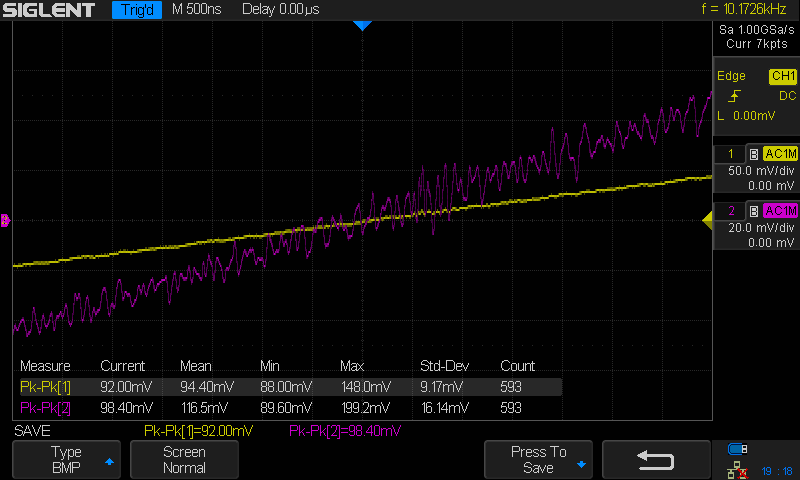
\includegraphics[width=7cm]{Osci/AvsfCC1n}
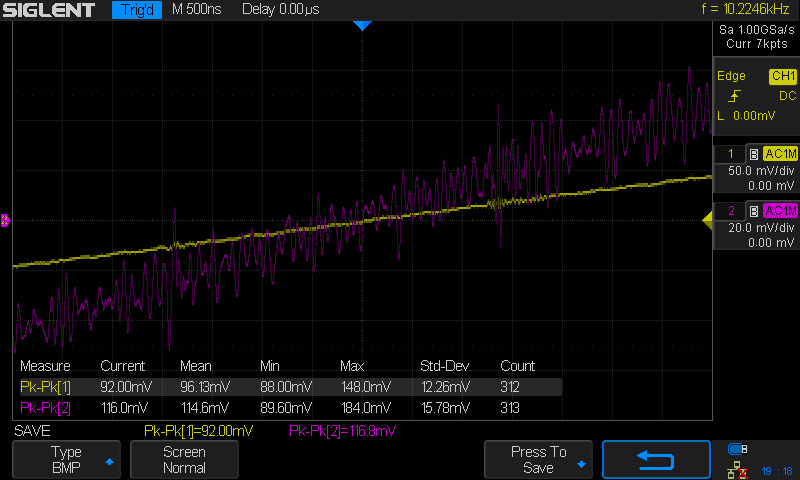
\includegraphics[width=7cm]{Osci/AvsfSinCC}
\caption{(De izquierda a derecha) Oscilogramas de \(V_o\) resultante de reemplazar el capacitor de compensacion de 220pF por (arriba): Un capacitor de 4.7pF, Un capacitor de 22pF, (abajo) Un capacitor de 1nF, Un circuito abierto} 
\label{fig:medCC}
\end{figure}

Se vario el capacitor de compensacion de forma similar a la simulacion del inciso \ref{sec:cc}, reemplazando el capacitor de 220pF por capacitores de menor y mayor valor y por un circuito abierto. Se observa que aparece un nivel de ruido producto de la oscilacion, el cual se reduce al aumentar el valor de \(C_c\). En los oscilogramas resultantes (fig \ref{fig:medCC}) se puede observar el aumento del nivel de ruido al reducir la capacidad, aunque este no es muy elevado en ninguna de las configuraciones. Esto es coherente con la simulacion, en la que al reducir \(C_c\) crece el sobrepico a alta frecuencia, aunque en el circuito real la amplitud de la oscilacion es mas acotada, probablemente debido a capacidades parasitas y a las limitaciones de ancho de banda de los transistores y los instrumentos.

\subsection{Variacion de R1 (11)} \label{sec:medR1}

\begin{figure}[ht] 
\centering
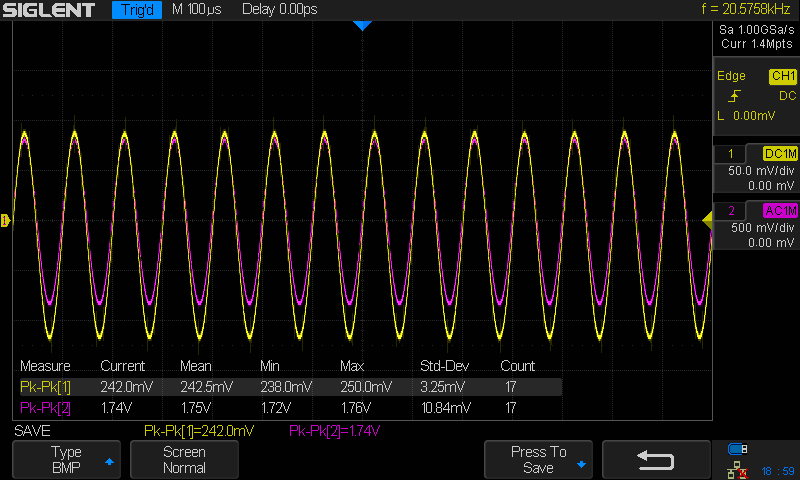
\includegraphics[width=5cm]{Osci/AvsfR1_6k8}
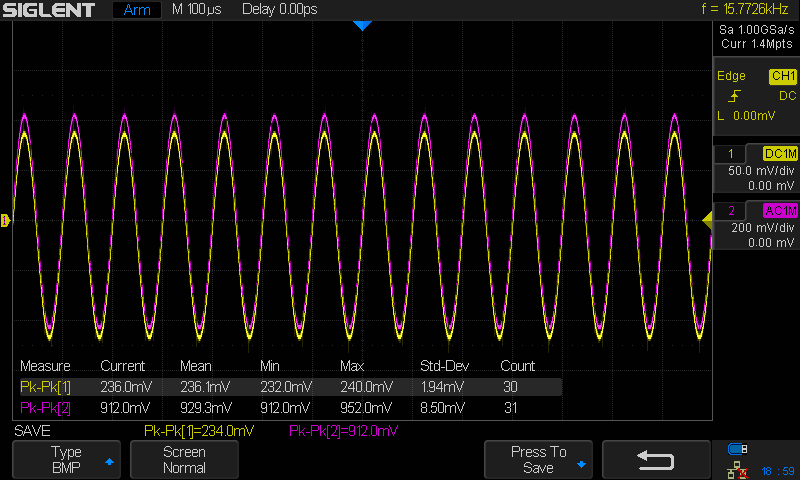
\includegraphics[width=5cm]{Osci/AvsfR1_15k}
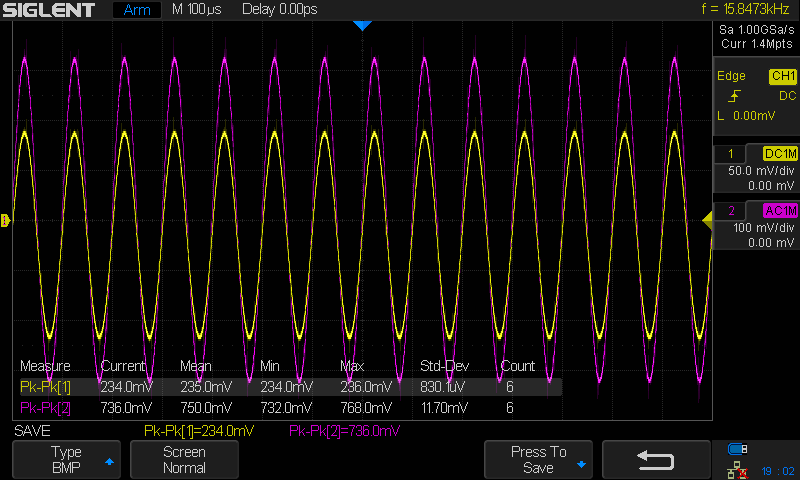
\includegraphics[width=5cm]{Osci/AvsfR1_22k}
\caption{(De izquierda a derecha) Oscilogramas de \(V_o\) resultante de reemplazar \(R_1\) de \(4.7K\Omega\) por recistencias de (De izquierda a derecha):  \(2.2K\Omega\), \(6.8K\Omega\), \(15K\Omega\) y \(22K\Omega\)}
\label{fig:medR1}
\end{figure}

Se vario la resistencia \(R_1\) de forma similar a la simulacion del inciso \ref{sec:simR1}. Se observa la variacion de la ganancia \(A_{vsf}\), medida de los oscilogramas (fig \ref{fig:medR1}), la cual aumenta al reducir \(R_1\) y disminuye al aumentarla, tal como predice la aproximacion \(A_{vsf} \approx 1 + \frac{R_2}{R_1}\). Los valores obtenidos se volcaron en la tabla comparativa (tab \ref{tab:R1}). Las diferencias respecto de los valores calculados y simulados llegan a aproximadamente 8\% en el peor caso (\(R_1 = 6.8K\Omega\)), lo cual puede atribuirse a las tolerancias de las resistencias utilizadas y al error de lectura de los oscilogramas.

\newpage
\subsection{\texorpdfstring{Medicion de \(R_{in}\) (12)}{Medicion de  (12)}}\label{sec:MedRin}

\begin{figure}[h!]
    \centering
    \includestandalone[width=11cm]{Rin}
    \caption{Circuito de medicion de Rin}
\label{fig:scheRin}
\end{figure}


\begin{figure}[!h] 
\centering
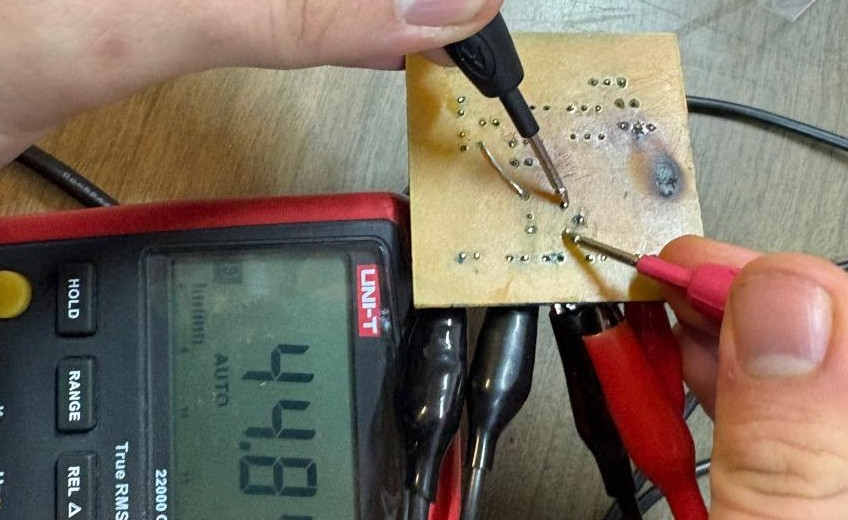
\includegraphics[width=11cm]{Fotos/Rin}
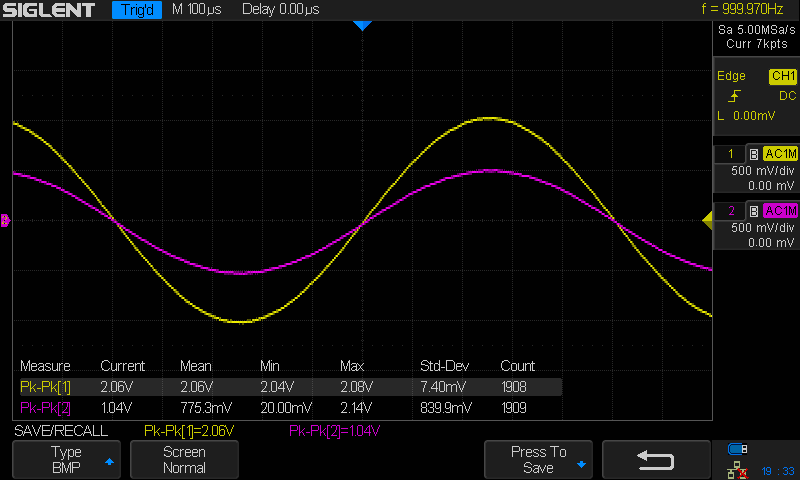
\includegraphics[width=11cm]{Osci/Rin}
\caption{Proceso de medicion de \(R_{in}\)}
\end{figure}

Para medir la \(R_{in}\) del circuito se conecto un potenciometro y voltimetro como se muestra en el esquematico (fig \ref{fig:scheRin}). El potenciometro forma junto con \(R_{in}\) un divisor de tension, por lo que la tension en la entrada del circuito es \(V_{in} = V_s \frac{R_{in}}{R_{pot} + R_{in}}\). Se ajusta el potenciometro hasta que la V medida se vuelve la mitad de la \(V_s\). A este punto se puede afirmar que \(R_{pot} = R_{in}\), el cual es posible medir. El valor obtenido (44.84K\(\Omega\)) se volco en la tabla comparativa (tab \ref{tab:xsf}). Dado que \(R_{isf}\) es de varios megaohms, lo que se mide en la practica es \(R_{in}\), y el resultado difiere en aproximadamente 5\% del valor nominal de 47K\(\Omega\), lo cual es compatible con la tolerancia tipica de una resistencia.


\newpage
\section{Tablas Comparativas de Valores (13)} 
A continuacion se vuelcan en las tablas comparativas los valores obtenidos en \ref{sec:calccc}, \ref{sec:simcc} y \ref{sec:medcc} (tab \ref{tab:cc}), \ref{sec:CalcXvsf}, \ref{sec:SimXvsf}, \ref{sec:MedAvsf} y \ref{sec:MedRin} (tab \ref{tab:xsf}) y \ref{sec:simR1} y \ref{sec:medR1} (tab \ref{tab:R1})

En cuanto al punto de operacion de continua, los valores calculados, simulados y medidos son consistentes entre si, con diferencias que pueden atribuirse a las tensiones de alimentacion reales, a las tolerancias de los componentes y a la dispersion de parametros de los transistores. La principal discrepancia es la corriente de colector de \(Q_2\) medida, que se discutio en la seccion de mediciones.

Respecto de los parametros de señal, la ganancia \(A_{vsf}\) presenta una concordancia de aproximadamente 1\% entre los tres valores, y \(R_{isf}\) queda dominada por \(R_{in}\), con diferencias de hasta 5\% atribuibles a la tolerancia de la resistencia. No se dispone de un valor medido de \(R_{osf}\), dado que su valor es del orden de las decimas de ohm, comparable a la resistencia de los cables y los contactos, lo cual dificulta su medicion directa. Por ultimo, al variar \(R_1\) la ganancia sigue la tendencia prevista por \(1 + \frac{R_2}{R_1}\), y la ganancia medida se mantiene dentro de aproximadamente 8\% de los valores calculados.

\begin{table}
\centering
\begin{tabular}{ |c|c|c|c| } \hline
Parametro       & Valor Calculado & Valor Simulado & Valor Medido \\ \hline         
\(V_{CE_{Q1}}\) &    9,08 V       &   9,15V        &  9,156V      \\ \hline 
\(V_{CE_{Q2}}\) &    9,08 V       &   9,02 V       &  8,851V      \\ \hline 
\(V_{CE_{Q3}}\) &    7,6 V        &   7,57 V       &  7,628V      \\ \hline 
\(V_{CE_{Q4}}\) &    1,35 V       &   1,32 V       &  1,308V      \\ \hline 
\(V_{CE_{Q5}}\) &   -8,35 V       &  -8,33 V       & -8,295V      \\ \hline 
\(V_{CE_{Q6}}\) &    9 V          &   8,97 V       &  8,892V      \\ \hline 
\(I_{C_{Q1}}\)  &    0,98 mA      &   0,91 mA      &  0.908mA     \\ \hline 
\(I_{C_{Q2}}\)  &    0,98 mA      &   1,09 mA      &  1,354mA     \\ \hline 
\(I_{C_{Q3}}\)  &    1,97 mA      &   2 mA         &  2,001mA     \\ \hline 
\(I_{C_{Q4}}\)  &    2.31mA       &   2,32 mA      &  2,396mA     \\ \hline 
\(I_{C_{Q5}}\)  &   -0,97 mA      &  -0,97 mA      & -0,9827mA    \\ \hline 
\(I_{C_{Q6}}\)  &    0,9 mA       &   0,9 mA       &  0,9207mA    \\ \hline 
\end{tabular}
\caption {Punto de operacion de continua}
\label{tab:cc}
\end{table}


\begin{table}
\centering
\begin{tabular}{ |c|c|c|c| } \hline
Parametro   & Valor Calculado & Valor Simulado    & Valor Medido      \\ \hline         
\(A_{vsf}\) & \(10.95\)       & \(10.96\)         & \(10.849\)        \\ \hline 
\(R_{isf}\) & \(47K\Omega\)   & \(46.47K\Omega\)  & \(44.84K\Omega\)  \\ \hline 
\(R_{osf}\) & \(170m\Omega\)  & \(155m\Omega\)    &                   \\ \hline 
\end{tabular}
\caption {Parametros de operacion de Señal}
\label{tab:xsf} 
\end{table}

\begin{table}
\centering
\begin{tabular}{ |c|c|c|c| } \hline
\(R_1\) [\(K\Omega\)] & \(A_{vsf}\) Calculado & \(A_{vsf}\) Simulado & \(A_{vsf}\) Medido \\ \hline         
2.2 & 22.36 & 22.19 & 21.438 \\ \hline 
4.7 & 11    & 10.95 & 10.849 \\ \hline 
6.8 & 7.91  & 7.88  & 7.310  \\ \hline 
15  & 4.13  & 4.12  & 3.949  \\ \hline 
22  & 3.13  & 3.13  & 3.196  \\ \hline 
\end{tabular}
\caption { \(A_{vsf}\) obtenido al variar \(R_1\)}
\label{tab:R1} 
\end{table}

\newpage
\section{Consideraciones Teoricas (14) y (15)}
El esquema de amplificacion realimentada cuenta con multiples ventajas con respecto a un esquema de lazo abierto. La ganancia es mas estable frente a variaciones en el circuito debidas a la dispersion de los parametros de los transistores o valores de las resistencias, es mas estable frente a alinealidades que introduzcan ruido distorsivo y es mas estable frente a variaciones en la carga del circuito. Adicionalmente permite controlar el valor de ganancia con la variacion de un unico componente. La resistencia de entrada aumenta y la de salida se reduce, ambos efectos siendo generalmente deseables para un amplificador de tension. Todas estas ventajas, sin embargo son apareadas con una perdida significativa de la ganancia de tension respecto a del amplificador a lazo abierto. Esta perdida es el costo de las mejoras mencionadas: la ganancia realimentada queda fijada principalmente por la red \(\beta\) y no por el amplificador, que debe tener una ganancia a lazo abierto lo suficientemente grande como para que \(A_{vs}\beta \gg 1\). Ademas, al reducirse la ganancia en un factor \(D\), el ancho de banda tiende a aumentar en un factor similar. Por otro lado, la realimentacion negativa puede transformarse en positiva a altas frecuencias debido al desfasaje de los polos del amplificador, lo que da lugar a sobrepicos u oscilaciones, motivo por el cual se utiliza el capacitor de compensacion analizado en las secciones anteriores.

El parametro realimentado (En este caso, \(V_f\)) se encuentra siempre en oposicion al parametro de entrada (\(V_s\)). Por otro lado corriente de entrada del circuito depende de la resistencia a lazo abierto y del parametro realimentado (\(V_i\)). De esta forma, \(V_f\) reduce \(V_i\) y por lo tanto \(I_e\) para una misma \(V_s\), aumentando la resistencia de entrada. Para cuantificar este efecto se parte de las definiciones de la corriente de entrada y de la resistencia de entrada realimentada, y se las iguala:

\begin{equation}
I_e = \frac{V_i}{R_{is}}
\end{equation}
\begin{equation}
R_(isf) = \frac{V_s}{I_e}
\end{equation}
\begin{equation}
I_e = \frac{V_s}{R_{isf}}
\end{equation}

\begin{equation}
\frac{V_s}{R_{isf}} = \frac{V_s - V_f}{R_{is}}
\label{eq:risf}
\end{equation}

Como puede observarse en (eq \ref{eq:risf}), por el efecto de \(V_f\), \(R_{isf}\) debera ser mayor a \(R_{is}\) para mantener la igualdad. Este se puede cuantificar de la siguiente manera:

\begin{equation}
\frac{R_{isf}}{R_{is}} = \frac{V_s}{V_i} = \frac{V_i + V_f}{V_i} =  \frac{V_i + A_v \beta V_i}{V_i} = 1 +A_v \beta
\end{equation}
\begin{equation}
{R_{isf}} = D{R_{is}}
\end{equation}

Es decir que la resistencia de entrada realimentada es \(D\) veces mayor que la resistencia de entrada sin realimentar. Con los valores de este circuito (\(D = 313.7\) y \(R_{is} = 22.27K\Omega\)) se obtiene una \(R_{isf}\) de varios megaohms. El razonamiento para la resistencia de salida es analogo: como la red de realimentacion muestrea la tension de salida, ante una variacion de la carga o una corriente que se extraiga de la salida, la tension \(V_o\) tiende a mantenerse constante porque la realimentacion corrige la señal de entrada. Esto equivale a una resistencia de salida menor, que resulta \(R_{osf} = \frac{R_{os}}{D}\). Por lo tanto, la topologia Tension-Serie aproxima el comportamiento de un amplificador de tension ideal, con resistencia de entrada elevada y resistencia de salida baja.

Debido a que \(I_{b2}\) es muy pequeña (del orden de los microamperes) la caida de tension en \(R_2\) sera practicamente nula, fijando la tension de continua \(V_o\). En terminos de retroalimentacion, en continua el \(\beta\) es unitario y por lo tanto la \(A_{vsf}\) tambien lo es, y al ser la \(V_s\) nula en continua, \(V_o\) resulta nula en continua. Esto se verifico en la medicion, donde se obtuvo una \(V_o\) de apenas 7.8mV. De esta forma el esquema de realimentacion tambien se utiliza en la determinacion del punto de trabajo del circuito, ya que fija la tension de salida y estabiliza la polarizacion de las etapas, evitando que dependa fuertemente de los parametros de los transistores.


\normalem
\end{document}